\documentclass{article}
\usepackage[utf8]{inputenc}
\usepackage{amsmath,amsthm,amssymb,scrextend,graphicx,framed}
\usepackage{fancyhdr}
\usepackage{listings}
\usepackage{tikz}
\usepackage{pgfplots}
\usetikzlibrary{calc,arrows.meta,positioning}
\tikzset{
    every node/.style={font=\sffamily\small},
    main node/.style={thick,circle,draw,font=\sffamily\Large,text width=1cm,align=center}
}
\DeclareMathOperator*{\argmax}{arg\,max}
\pagestyle{fancy}
\author{Joss Moffatt}
\title{The Urinal Problem}
\begin{document}
\begin{titlepage}
  \begin{center}
    \huge
    \textbf{The Urinal Problem}\\
    \vspace{1cm}
    \textbf{Joss Moffatt}\\
    \large
    \vspace{1cm}
    \includegraphics[height=50mm]{University-Logo/UOM.png}\\ % Include a department/university logo - this will require the graphicx package
    \vspace{1cm}
    University of Manchester\\
    Christmas 2019
    \vspace{1cm}
    \begin{abstract}
      Consider a person walks into a male bathroom with $n$ urinals and $\Phi$ is the set of free urinals and $\Xi$ is the set of occupied ones, where should this person go to maximise their privacy? I demonstrate an algorithm to select the most appropriate urinal in linear time and propose a new extension to the original problem.  
    \end{abstract}
   \end{center}
\end{titlepage}
\maketitle
\tableofcontents

\pagebreak
\vspace{1cm}
\lhead{Section \thesection}
\rhead{Joss Moffatt}
\cfoot{\thepage}
\section{Introduction}
Typically when walking into the men's bathroom urinals appear on the immediate wall, evenly spaced and without separators providing instant privacy. Under these constraints, a somewhat natural heuristic takes effect and we use this to perform the selection of which urinal we wish to go to. In the short mockumentary \textit{"Male Restroom Etiquette"} by Phil R. Rice  [Zarathustra Studios, 2006] the section called Urinal Selection explores the common selection heuristic: 
\begin{quote}
    "Always select the urinal that is as far away as possible from men who are using other urinals."
\end{quote}
In pursuing this approach, assuming $P_{1}$ is at urinal 1 and there are 5 urinals, then $P_{2}$ would try and maximise his distance from $P_{1}$ and this results in him picking urinal 5. If a third person $P_{3}$ enters he has to maximise the distance between him, $P_{1}$ and $P_{2}$ so naturally picks urinal 3. This results in the configuration seen in Figure 1.
\begin{figure}[h]
\centering
  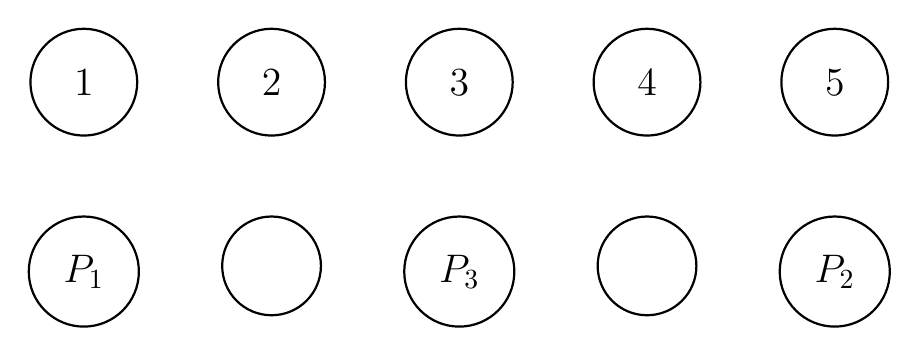
\begin{tikzpicture}[->,>={Stealth[round,sep]},shorten >=1pt,auto,node distance=1cm]

    \node[main node] (1) {$1$};
    \node[main node] (2) [right =of 1]{$2$};
    \node[main node] (3) [right =of 2]{$3$};
    \node[main node] (4) [right =of 3]{$4$};
    \node[main node] (5) [right =of 4]{$5$};
    \node[main node] (6) [below =of 1]{$P_{1}$};
    \node[main node] (6) [below =of 2]{};
    \node[main node] (6) [below =of 3]{$P_{3}$};
    \node[main node] (6) [below =of 4]{};
    \node[main node] (6) [below =of 5]{$P_{2}$};
  \end{tikzpicture}
\caption{Uncompleted for $n=5$} \label{fig:M1}
\end{figure}
\begin{figure}[h]
\centering
  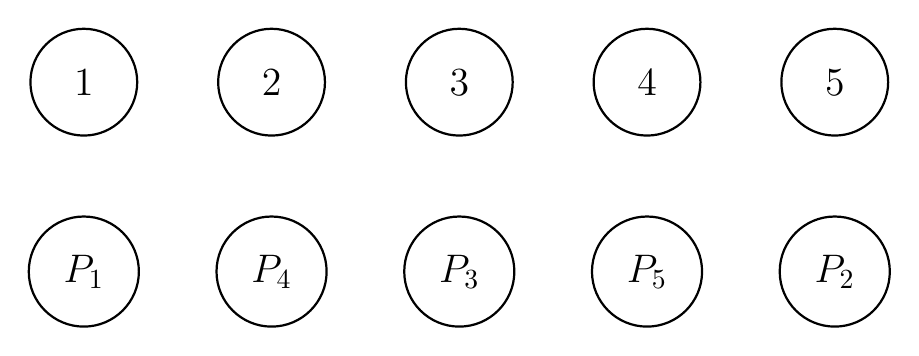
\begin{tikzpicture}[->,>={Stealth[round,sep]},shorten >=1pt,auto,node distance=1cm]

    \node[main node] (1) {$1$};
    \node[main node] (2) [right =of 1]{$2$};
    \node[main node] (3) [right =of 2]{$3$};
    \node[main node] (4) [right =of 3]{$4$};
    \node[main node] (5) [right =of 4]{$5$};
    \node[main node] (6) [below =of 1]{$P_{1}$};
    \node[main node] (6) [below =of 2]{$P_{4}$};
    \node[main node] (6) [below =of 3]{$P_{3}$};
    \node[main node] (6) [below =of 4]{$P_{5}$};
    \node[main node] (6) [below =of 5]{$P_{2}$};
  \end{tikzpicture}
\caption{Completed for $n=5$} \label{fig:M2}
\end{figure}
\\\\However we now fall into a problem. Now if $P_{4}$ tries to select a urinal, both urinal 2 and 4 are the optimal choices, therefore we should define an extension to our original heuristic to always allow a full configuration of people at urinals. Due to the laziness of most people, if there is a set of urinals that are equally optimal, then a person will choose the closest one to the door. Consequently our updated heuristic is:
\begin{quote}
    "Always select the urinal that is as far away as possible from men who are using other urinals. If there are multiple optimal urinals, choose the closest one to the door."
\end{quote}
If we presume the distance to the door is proportional to the number of the toilet our final configuration for $n=5$ is that seen in Figure 2. 

\section{Formalising the Selection}
Clearly, under our current definition, we have a set of urinals this set is compromised of 2 disjoint sets of urinals. These sets are the occupied urinals and the free urinals. Consequently, we can now formally define these sets.
\begin{framed}
  \section*{Set of Urinals}
    The set of all urinals $U$ is equal to the union of the disjoint sets, the set of free urinals $\Phi$ and the set of occupied urinals $\Xi$:
    \begin{itemize}
        \item $U = \Phi \cup \Xi$.
        \item $\Phi \cap \Xi = \emptyset$.
        \item $\left|\Phi\right| \geq 0$.
        \item $\left|\Xi\right| \leq \left|U\right|$.
        \item $\left|\Xi\right| + \left|\Phi\right| \equiv \left|U\right|$ 
    \end{itemize}
\end{framed}
Further analysing the current definition it is clear that a function must be defined that takes a selected urinal position and the occupied urinals and returns the number of urinals away between the selected one and its nearest occupied neighbours. We will define this as the adjacent neighbour distance function.
\subsection{Adjacent Neighbour Distance Function}
\begin{framed}
    \section*{Adjacent Neighbour Distance Function}
      The Adjacent Neighbour Distance function $\delta(u, \Xi)$:
      \begin{itemize}
          \item $u$ is the selected urinal, $u \in \Phi$.
          \item $\Xi$ is the set of occupied urinals.
          \item $\delta(u, \Xi) = \min(\{x \mid x = \left| n - u \right| , \forall n \in \Xi\})$ .
          \item $\delta(u, \Xi) \in [1, n]$ .
      \end{itemize}
  \end{framed}
The Adjacent Neighbour Function returns the minimum distance from the selected urinal to its closest occupied neighbour. Therefore our definition of $\delta$ is valid as we are getting the absolute distance from the selected urinal to all the others and then finding the minimum value from this newly constructed set of distances. This works clearly as the minimum absolute distance from the all the occupied urinals will be its closest adjacent neighbour and hence the closest adjacent distance. \hfill\qedsymbol\\\\
Next, we want to find the set of urinals that maximise the adjacent neighbour distance function in order to maximise the person's privacy. Then we wish to find the minimum of the resulting set such that one may satisfy the closest to the door clause in the updated heuristic definition. Taking into account all of this, we can then produce our selection function.
\subsection{Selection Function}
Using Schmidt's  definition for the \textit{argmax} function [Schmidt, 2016]:
\begin{quote}
    We define the $argmax$ of a function $f$ defined on a set $D$ as:
    \centering
    $\argmax_{x \in D} f(x) = \{x \mid f(x) \geq f(y), \forall y \in D\}$

\end{quote}
\begin{framed}
    \section*{Selection Function}
      The Selection function $\sigma(\Xi, \Phi)$:
      \begin{itemize}
          \item $\Xi$ is the set of occupied urinals.
          \item $\Phi$ is the set of free urinals.
          \item $\sigma(\Xi) = \min(\argmax_{u \in \Phi} \delta(u, \Xi))$.
          \item $\sigma(\Xi) \in \Phi$.
      \end{itemize}
  \end{framed}
Proving this algorithm is correct again is trivial, we are finding the argument that maximises our \textit{Adjacent Neighbour Distance Function} and then getting the smallest of these arguments. This is then the closest urinal to the door that maximises distance between adjacent neighbours which is the optimal selection given our updated heuristic definition. \hfill\qedsymbol
\section{Algorithms}
\subsection{Quadratic Time Algorithm}
One can simply convert our algorithms into python for it to resemble our \textit{Selection function}. In our algorithm F represents $\Phi$ and O represents $\Xi$ so by iterating over $\Phi$ and recording the greatest distances from the \textit{Adjacent Neighbour Distance function} and then finding the minimal from the output set which is the same process as our $\sigma$ function so our algorithm is valid.\hfill\\
\begin{center}
    \begin{lstlisting}
      def adjacent_neighbour_distance(u, O):
        for index, value in enumerate(O):
          if value > u:
            # O(1) due to the constant size
            return min(abs(O[index - 1] - u), abs(O[index] - u))
        return min(abs(O[- 1] - u), abs(O[-2] - u))
        
      def selection(O, F):
        max_args = []
        max_dist = 0
        for index, u in enumerate(F):
          distance = adjacent_neighbour_distance(u, O)
          if distance > max_dist:
            max_dist = distance
            max_args = [u]
          elif distance == max_dist:
            max_args.append(u)
          else:
            continue
        return min(max_args)
    \end{lstlisting}
\end{center}
However, one can clearly see that our function representing $\delta$ is $O(p)$ where $p$ is the size of the input set $\Xi$. This is as you iterate over the input array until the current urinal number is greater than the selected urinal and then returns the minimum distance between the selected urinal and the urinals surrounding it. By considering the condition to check that the current urinal number is greater than the selected one allows the best case time complexity to be $O(1)$ however, worst and average case complexity is still $O(p)$.\\\\
In the selection algorithm we then iterate over the input set and if we say the size of $\Phi$ is $m$ then we perform the iteration within the selection function $m$ times. In this loop we only do constant time operations apart from the distance calculation, which we previously established is $O(p)$. By applying the product rule for asymptopic analysis the loop has an overall complexity of $O(pm)$. We then return the minimum of the resulting final set which has a worst case time complexity of $O(m)$ which only occurs when the $\argmax_{u \in \Phi} \delta(u, \Xi) = \Phi$ so we will then have to do $m$ checks to find the minimum value. Finally we can conclude that $\sigma \in O(pm)$ but as $p$ and $m$ are completely reliant on the total number of urinals $n$ due to the equality $\left|\Xi\right| + \left|\Phi\right| \equiv \left|U\right|$ we can conclude that $\sigma$ runs in quadratic time with regards to the total number of urinals then $\sigma \in O(n^2)$\\\\
In a paper on the Urinal Problem (Kranakis and Krizanc, 2019) for a non-empty initial configuration, it is made clear you can generate an algorithm in $O(n^2)$ as we have done. But, they further conjecture that there will be an algorithm that can select the optimal urinal in linear time. However, using our definition for $\sigma$ we are having to find a globally optimal solution for a function that runs in linear time already by iterating over all the values and recording the maximum. This approach will always run in quadratic time and in order to reduce our time complexity to linear time we will have to find a better way to optimise our system.
 
\subsection{Linear Time Algorithm}
Crucially, we need to find a better way of finding the optimal solution without having to check each individual value. Consequently, consider the following configuration:
\begin{figure}[h]
    \centering
      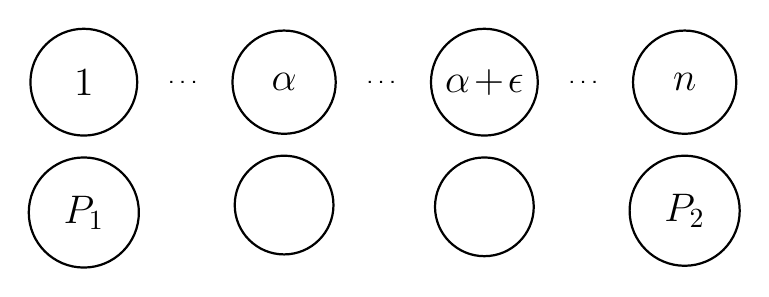
\begin{tikzpicture}[->,>={Stealth[round,sep]},shorten >=1pt,auto,node distance=0.25cm]
    
        \node[main node] (1) {$1$};
        \node  (2) [right =of 1]{\ldots};
        \node[main node] (3) [right =of 2]{$\alpha$};
        \node  (4) [right =of 3]{\ldots};
        \node[main node] (5) [right =of 4]{$\alpha + \epsilon$};
        \node  (6) [right =of 5]{\ldots};
        \node[main node] (9) [right =of 6]{$n$};
        \node[main node] (6) [below =of 1]{$P_{1}$};
        \node[main node] (6) [below =of 3]{};
        \node[main node] (6) [below =of 5]{};
        \node[main node] (6) [below =of 9]{$P_{2}$};
      \end{tikzpicture}
    \caption{Configuration where largest gap between occupied urinals is $\epsilon$} \label{fig:M3}
\end{figure}
There exists a urinal $\alpha$ where the gap between it and the urinal to its right is $\epsilon$ is the greatest gap in the system. By considering how our heuristic was defined, we know that we are trying to maximise the distance between the person who is choosing a urinal and the adjacent neighbours. Consequently this the gap between the urinals $\alpha$ and $\alpha + \epsilon$ is where the person wants to go as it will guarantee to maximise their privacy. Therefore when 1,$ n \in \Xi$ the person will want to go at the position $\alpha + \lfloor\epsilon / 2\rfloor$ \- the floor function is used in order to consider the distance element of the heuristic. The value $\lfloor\epsilon / 2\rfloor$ is effectively the optimal $distance$ value for the \textit{Adjacent Neighbour Distance function} as it is the maximum distance you can possibly achieve bewteen adjacent neighbours in the system. However, instead of taking $O(n^2)$ to solve we can reduce this to $O(n)$ by iterating over the set of occupied urinals and then finding the gap between consecutive urinals and recording $\alpha$ and $distance$ when a \textit{new} max $distance$ is found. Note we must only record at a new max distance again in order to consider the distance element of the heuristic.\\\\
Next we must consider if there are runs of free urinals at the start starting from urinal 1, for example:\\
\begin{center}
    $\Phi = \{1,2,3,4,5,7....\}$ 1,2,3,4,5 would be the run at the start as 6 is occupied
\end{center}
or the end of the set, ending at n:\\
\begin{center}
    $\Phi = \{... n-3,n-1,n\}$ n-1, n would be the run at the end as n-2 is occupied
\end{center}
It is important to do this as these pseudo-gaps  will not show up when calculating the distance between the occupied urinals as they are clearly not occupied but are technically still gaps as they can be occupied. This is easily worked around as if there is a run of length $s$ at the start,a run of length $e$ at the end,if $s \geq \lfloor\epsilon / 2\rfloor$ and $s \geq e$ then it will want to go at urinal number one as it is the new distance away from any urinal and then urinal 1 is the optimal urinal. Conversely if $e > \lfloor\epsilon / 2\rfloor$ and $e > s$ then the end run is then the biggest distance away from any urinal and hence last urinal is the optimum choice.\\\\
\begin{center}
    \begin{lstlisting}
    def efficient_selection(O, F):
      distance = 0
      urinal_choice = -1
      alpha = 0
      for index in range(len(O) - 1):
        if distance < int((O[index+1] - O[index]) / 2):
          distance = int((O[index+1] - O[index]) / 2)
          alpha = O[index]
      start_run = O[0] - F[0]
      end_run = F[-1] - O[-1]
      if (start_run >= end_run) and (start_run >= distance):
        return  F[0]
      elif (end_run > start_run) and (end_run > distance):
        return F[-1]
      else:
        max_gap_center = alpha + distance
        closest_value = 2 * distance
        for index, value in enumerate(F):
          if closest_value > abs(value - max_gap_center):
            closest_value = abs(value - max_gap_center)
            urinal_choice = F[index]
        return urinal_choice
    \end{lstlisting}
\end{center}
Analysing Figure 5, all operations are $O(1)$ apart from the loops. The first is iterated over $p-1$ times, again where $p$ is the size of $\Xi$, and the second is iterated $m$ times, where $m$ is the size of $\Phi$. In the best case where there is a long run at the start or end, the second loop is never even reached so we have the best case time complexity, therefore, it is $O(p)$. For the worst case it $\max(O(p), O(m))$ but as discussed before as both $p$ and $m$ dependant on the overall number of urinals $n$ we have best, average and worst-case time complexity of $O(n)$ which then proves there is an algorithm to optimally choose a urinal in polynomial time.
\subsection{Comparing the Algorithms}
Figure 6 shows the time taken to select an optimal solution for an increasing number of urinals where the number of occupied urinals is randomly chosen and the free urinals are then calculated from that. The linear time algorithm is barely visible as it is so close to the x axis whilst the quadratic algorithm is tending towards a $n^2$ relationship which is what we expect, but the more efficient algorithm is clearly performing very well as the time taken is barely increasing even with 10000 urinals.
\begin{figure}[h]
\centering
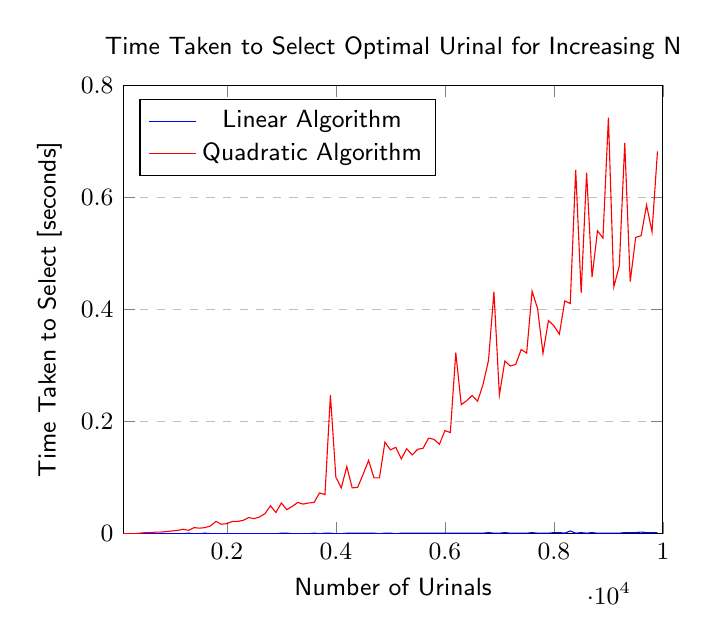
\begin{tikzpicture}
\begin{axis}[
    title={Time Taken to Select Optimal Urinal for Increasing N},
    xlabel={Number of Urinals},
    ylabel={Time Taken to Select [seconds]},
    xmin=100, xmax=10000,
    ymin=0, ymax=0.8,
    legend pos=north west,
    ymajorgrids=true,
    grid style=dashed,
]
 
\addplot[
    color=blue,
    ]
    coordinates {
    (100,0.0)(200,0.0)(300,0.0)(400,0.0)(500,0.0)(600,0.0)(700,0.0)(800,0.0)(900,0.0)(1000,0.0)(1100,0.0)(1200,0.0)(1300,0.0009961128234863281)(1400,0.0)(1500,0.0)(1600,0.0010335445404052734)(1700,0.0)(1800,0.0)(1900,0.0)(2000,0.0)(2100,0.0)(2200,0.0)(2300,0.0)(2400,0.0)(2500,0.0)(2600,0.0)(2700,0.0)(2800,0.0)(2900,0.0)(3000,0.0009968280792236328)(3100,0.000997304916381836)(3200,0.0)(3300,0.0)(3400,0.0)(3500,0.0)(3600,0.000997781753540039)(3700,0.0)(3800,0.0009374618530273438)(3900,0.0009975433349609375)(4000,0.0)(4100,0.0)(4200,0.0009989738464355469)(4300,0.0009570121765136719)(4400,0.0009963512420654297)(4500,0.000997781753540039)(4600,0.0009942054748535156)(4700,0.0009970664978027344)(4800,0.0)(4900,0.000997781753540039)(5000,0.0009965896606445312)(5100,0.0)(5200,0.000997304916381836)(5300,0.0009951591491699219)(5400,0.0009963512420654297)(5500,0.0009963512420654297)(5600,0.0009965896606445312)(5700,0.0010402202606201172)(5800,0.0009975433349609375)(5900,0.0009970664978027344)(6000,0.0009975433349609375)(6100,0.000997781753540039)(6200,0.0009975433349609375)(6300,0.0009968280792236328)(6400,0.0009965896606445312)(6500,0.0009975433349609375)(6600,0.0009944438934326172)(6700,0.0009968280792236328)(6800,0.0019986629486083984)(6900,0.0009965896606445312)(7000,0.0009996891021728516)(7100,0.0019948482513427734)(7200,0.0009579658508300781)(7300,0.000997781753540039)(7400,0.000997304916381836)(7500,0.0009965896606445312)(7600,0.001989603042602539)(7700,0.0009968280792236328)(7800,0.000997781753540039)(7900,0.000997304916381836)(8000,0.001984834671020508)(8100,0.001994609832763672)(8200,0.0010378360748291016)(8300,0.004987001419067383)(8400,0.000997304916381836)(8500,0.0019948482513427734)(8600,0.0009970664978027344)(8700,0.0020287036895751953)(8800,0.0009357929229736328)(8900,0.0009882450103759766)(9000,0.0009965896606445312)(9100,0.0009946823120117188)(9200,0.0009975433349609375)(9300,0.001995086669921875)(9400,0.002016782760620117)(9500,0.001951456069946289)(9600,0.0029914379119873047)(9700,0.0019948482513427734)(9800,0.0020363330841064453)(9900,0.0020220279693603516)
    };
 \addplot[
    color=red,
    ]
    coordinates {
    (100,0.0)(200,0.0)(300,0.0)(400,0.0009946823120117188)(500,0.001995086669921875)(600,0.001998424530029297)(700,0.0029876232147216797)(800,0.0029916763305664062)(900,0.003989458084106445)(1000,0.00498652458190918)(1100,0.006021976470947266)(1200,0.008019685745239258)(1300,0.0059850215911865234)(1400,0.010933160781860352)(1500,0.009930610656738281)(1600,0.010971784591674805)(1700,0.013925552368164062)(1800,0.021941184997558594)(1900,0.01695394515991211)(2000,0.017951488494873047)(2100,0.021940946578979492)(2200,0.021943092346191406)(2300,0.02397751808166504)(2400,0.028882741928100586)(2500,0.026888370513916016)(2600,0.02991962432861328)(2700,0.0359039306640625)(2800,0.049870967864990234)(2900,0.037859201431274414)(3000,0.05485391616821289)(3100,0.04288530349731445)(3200,0.04886960983276367)(3300,0.05588984489440918)(3400,0.052863121032714844)(3500,0.054895877838134766)(3600,0.05580759048461914)(3700,0.07284307479858398)(3800,0.06983518600463867)(3900,0.24733805656433105)(4000,0.10077285766601562)(4100,0.08178353309631348)(4200,0.11979794502258301)(4300,0.08178448677062988)(4400,0.08278083801269531)(4500,0.10618400573730469)(4600,0.13085055351257324)(4700,0.0996696949005127)(4800,0.09973311424255371)(4900,0.16356396675109863)(5000,0.14963960647583008)(5100,0.15415596961975098)(5200,0.13364148139953613)(5300,0.1516406536102295)(5400,0.14062714576721191)(5500,0.15059781074523926)(5600,0.15256977081298828)(5700,0.17052435874938965)(5800,0.16850519180297852)(5900,0.15957331657409668)(6000,0.18401336669921875)(6100,0.18056035041809082)(6200,0.32312536239624023)(6300,0.23032069206237793)(6400,0.23740887641906738)(6500,0.24680185317993164)(6600,0.23641133308410645)(6700,0.2663273811340332)(6800,0.3091104030609131)(6900,0.4318840503692627)(7000,0.24734282493591309)(7100,0.30811548233032227)(7200,0.2994041442871094)(7300,0.3021233081817627)(7400,0.3287200927734375)(7500,0.32218170166015625)(7600,0.43280649185180664)(7700,0.4020695686340332)(7800,0.32183384895324707)(7900,0.38049960136413574)(8000,0.371021032333374)(8100,0.3560471534729004)(8200,0.41539812088012695)(8300,0.4108388423919678)(8400,0.6492612361907959)(8500,0.42985033988952637)(8600,0.6443278789520264)(8700,0.45786070823669434)(8800,0.540579080581665)(8900,0.5275967121124268)(9000,0.7425687313079834)(9100,0.44043898582458496)(9200,0.4781668186187744)(9300,0.6972768306732178)(9400,0.4498410224914551)(9500,0.5286014080047607)(9600,0.5318183898925781)(9700,0.5864307880401611)(9800,0.5387005805969238)(9900,0.6822967529296875)
    };
    \legend{Linear Algorithm, Quadratic Algorithm}
\end{axis}
\end{tikzpicture}
\caption{Graph comparing the algorithms} \label{fig:M4}
\end{figure}
\vspace{1cm}
\section{Extensions to the Theme}
\subsection{The Infinite Bathroom}
Consider a bathroom with a total number of urinals which tends towards $\infty$. We then encounter the problem that in an empty configuration the first person would choose the first urinal, but then based on the algorithm, the next person would choose the last toilet. However, it would take a \textbf{very} long time to get to the last toilet in this case - you would never get there. When this happens our algorithm starts to fail as we are assuming getting to the toilet is inexpensive and we can somehow just magically teleport there. Consequently, I conjecture there is a value $\kappa$ that will serve as an optimum threshold. This will mediate how the algorithm predicts the optimal urinal, as now getting to the urinal will be expensive and as the number of urinals tends towards some large number it would be more optimal to travel only a certain distance.
\section{Bibliography}
\begin{itemize}
  \item Kranakis, E. and Krizanc, D. (2019). The Urinal Problem. [ebook] Available at: https://people.scs.carleton.ca/~kranakis/Papers/urinal.pdf (Accessed 24 Dec. 2019).
  \item Schmidt, M. (2016). Argmax and Max Calculus. [ebook] UBC, p.1. Available at: https://www.cs.ubc.ca/~schmidtm/Documents/2016\_540\_Argmax.pdf (Accessed 21 Dec. 2019).
  \item Zarathustra Studios. (2006). Male Restroom Etiquette. [Online]. available at: https://www.youtube.com/watch?v=IzO1mCAVyMw (Accessed: 21 December 2019).
\end{itemize}
\end{document}